\begin{adjustbox}{width=\textwidth}
	\begin{tikzpicture}[every node/.style={inner sep=0,outer sep=0}]
	
		\node [anchor=north west] (imgSpalten) at (0,0) {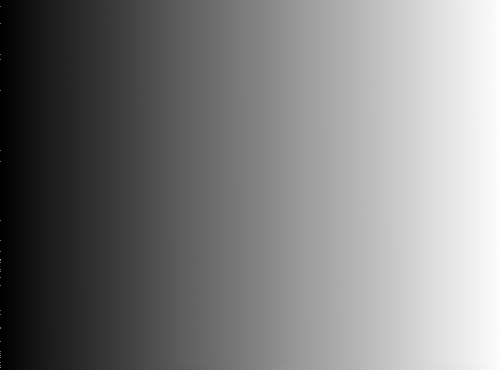
\includegraphics[width=.47\textwidth]{04_deflektometrischeRegistrierung/auswertungDeflektometrischeRegistrierung/figures/spaltenRegistrierung_optimal}};
		\node [below=0.2cm of imgSpalten] {Graubild der Spaltenzuordnung \acrshort{frx}$(x,y)$};
		\node [anchor=north west] (imgZeilen) at (0.53\textwidth,0) {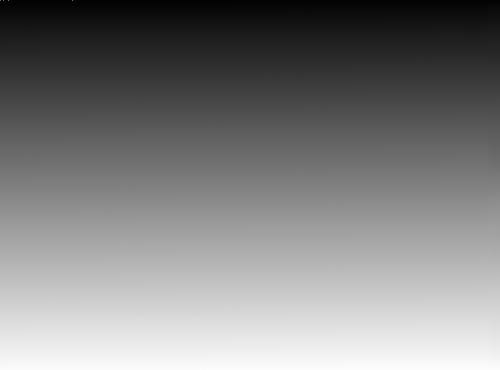
\includegraphics[width=.47\textwidth]{04_deflektometrischeRegistrierung/auswertungDeflektometrischeRegistrierung/figures/zeilenRegistrierung_optimal}};
		\node [below=0.2cm of imgZeilen] {Graubild der Zeilenzuordnung \acrshort{fry}$(x,y)$};
	
	\end{tikzpicture}
\end{adjustbox}
\caption[Darstellung Spalten- und Zeilenregistrierung]{Darstellung der Spalten- und Zeilenregistrierung als Bilder in Graustufen mit $I_{min} = 0$ und $I_{max} = 255$. Je dunkler ein Pixel ist, desto weiter links bzw. oben befindet sich die zugeordnete Spalten- bzw. Zeilenposition.}